\documentclass[12pt]{article}

\setlength{\topmargin}{-.5in}
\setlength{\textheight}{9in}
\setlength{\oddsidemargin}{.125in}
\setlength{\textwidth}{6.25in}
\usepackage{amsmath}
\usepackage{verbatim}
\usepackage{graphicx}
\newcommand{\TODO}[1]{\textcolor{red}{\textbf{[TODO:#1]}}}
\usepackage{listings}
\usepackage{color}
\usepackage{url}
\usepackage{syntax}
  \usepackage{tabularx}
  \usepackage{graphicx}
\definecolor{gray}{rgb}{0.5,0.5,0.5}
\definecolor{mauve}{rgb}{0.58,0,0.82}
\usepackage{amsmath}
\usepackage{verbatim}
\usepackage{graphicx}
\usepackage{hyperref}
\begin{document}

\begin{titlepage}

\begin{figure}[t]
    \centering
    
\includegraphics[scale=0.4]{./draws/inria-logo.png}
\end{figure}

\vspace*{2cm}
\begin{center}
	{\huge \textbf{VerCors v4 Tutorial}} \vspace*{1cm}
\\
    {\large INRIA – Sophia-Antipolis } \medskip \\
\end{center}

%
\vfill
\begin{center}
\begin{minipage}[b]{0.5\textwidth}
    \vspace*{1.3cm}
    \begin{center}
        {\large September 2016}
    \end{center}
        \begin{center}
        {\large oleksandra.kulankhina@gmail.com \\
        \large eric.madelaine@inria.fr}
    \end{center}
     \vspace*{1cm}
        \begin{center}
        {\large VCE version 4.1.1}
    \end{center}
\end{minipage}%
\end{center}

\thispagestyle{empty}

\end{titlepage}

\tableofcontents
\newpage

\section{Brief overview}\label{sec:intro}
This document helps the developers of the VerCors platform in understanding the project architecture and provides simple steps to configure their local workspace. 

Here we provide a very brief overview of the used technologies. References to all the necessary resources are listed in Section~\ref{sec:refs}. 
The VerCors platform represents a set of plug-ins for the Eclipse IDE. It includes graphical designers for the architecture and behaviour of GCM components. All the designers are based on the Sirius (Obeo designer) technology which is, in its turn, based on EMF and GMF. VerCors includes the source code of the Obeo UML designer for the management of UML elements. In addition, VerCors includes plug-ins generating Java code of the modelled application and plug-ins generating an input for the CADP model-checker. The source code of VerCors is stored in an SVN repository, the examples are stored on GitHub. VerCors is a Maven project with several modules where each module is one of the plug-ins. The project is continuously built on a Jenkins server. 

\section{Configuring the workspace}
\begin{enumerate}
\item
Download and install Obeo Designer community version: \url{http://www.obeodesigner.com/download}. Obeo designer is based on Eclipse IDE, hence, it includes all standard functionalities of Eclipse. If you are not familiar with Eclipse IDE, the following url will help you to get the basic information: \url{https://www.eclipse.org/users/}
\item
Use Eclipse Marketplace in order to install the following plug-ins on top of Obeo Designer: 
	\begin{enumerate}
	\item
	Subversive SVN team provider: \url{http://marketplace.eclipse.org/content/subversive-svn-team-provider}
	\item
	Maven integration for Eclipse: \url{http://marketplace.eclipse.org/content/maven-integration-eclipse-juno-and-newer}
	\end{enumerate}
\item
Install the Eclipse plug-ins for the UML meta-model. In the toolbar on the top of Eclipse select \texttt{Help -> Install new Software}. This will open a wizard. In the \texttt{Work with} textfield select \texttt{Obeo Designer Community Edition} as illustrated in Figure~\ref{fig:install-uml}. A list of software to be installed should appear. Select \texttt{Obeo Designer Community Edition - Extentions -> UML 2 Extender SDK} and finalise the procedure.
\end{enumerate}


\begin{figure}
\centering
    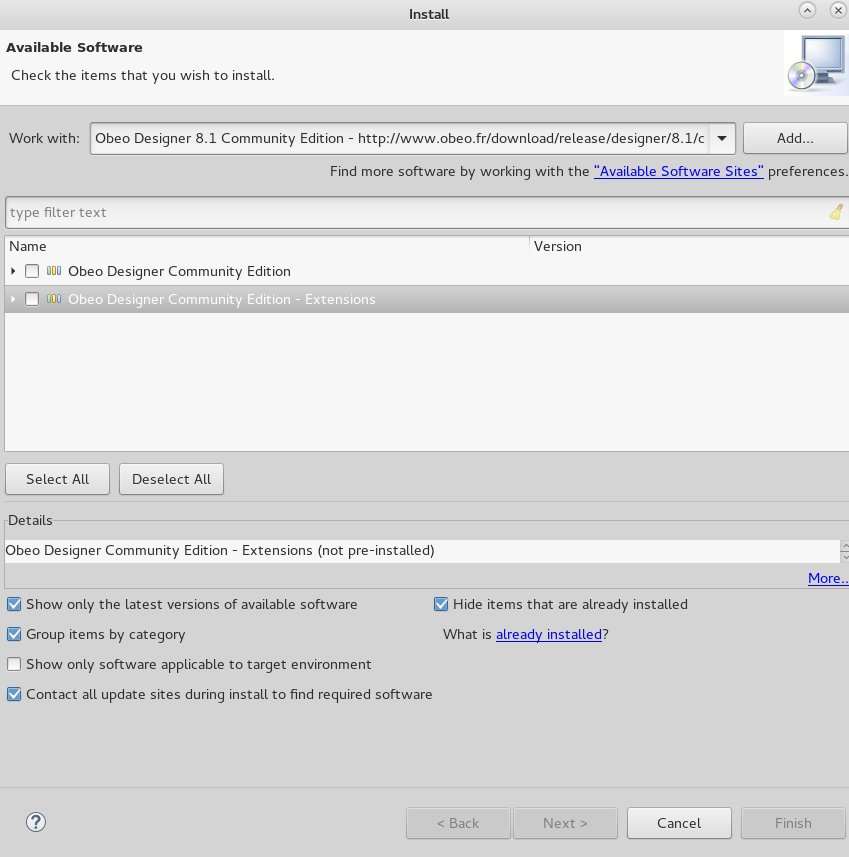
\includegraphics[width=11cm]{draws/install-uml.jpg}
 \caption{Installation of UML meta-model plug-ins}
  \label{fig:install-uml}
\end{figure}

\paragraph{Important! If you already have an Obeo Designer with VerCors installed, please, use another installation of Obeo Designer for working with the source code.}

\section{Working with SVN}
\subsection{Checkout}

All the source files are stored at INRIA GForge. At \url{https://gforge.inria.fr/scm/?group_id=193} the developer can find all the information required to successfully checkout the project.

\paragraph{Access.} If you checkout the project anonymously, you will not be able to commit modifications. Moreover, in order to be able to commit in the repository, the developer should have such a right provided by one of the administrators of the repository. Hence, if you are a developer, use either a \textbf{developer access} method or access the repository via ssh.

\paragraph{Eclipse Subversive.} In order to keep things coherent, we suggest using Eclipse Subversive for all operations with SVN. The following web-page provides the references to the documentation: \url{https://eclipse.org/subversive/documentation.php}. If you have issues with checking-out the project, make sure you have an SVn connector installed or trying changing it to another one. More about SVN connectors: \url{https://polarion.plm.automation.siemens.com/products/svn/subversive}.

\paragraph{} The current version of VerCors includes several branches and the most important ones are:
\begin{itemize}
\item
\texttt{/branches/Vercors/VCEv3Sirius/vceSirius1.0} - the main branch used for the build
\item
\texttt{/branches/Vercors/VCEv4-OpenPNets} - the branch for working with open pNets
\end{itemize} 

\subsection{Commit}

Before committing, please, choose carefully the commit message and increase the version of VerCors as explained in~\ref{sec:versioning}. If the committed changes do not affect the business logic of the application (e.g. the changes to the documentation), then the version should not be incremented.

\paragraph{Important! Please, do NOT commit the \texttt{bin} folders and all the files related to the local build.}


\section{Versioning}
\label{sec:versioning}

VerCors fallows \texttt{x.y.z} versioning standard, where:
\begin{itemize}
\item[x]
 – is always number '4'. It can be incremented if the underlying technology is completely changed.
\item[y]
 – is incremented only for major change
\item[z]
 – is incremented for bug fix
 \end{itemize}

\section{Running VerCors from the source code}

During the development, the programmer often needs to run his application from the source code. In order to run VerCors from the source code, you should follow a standard procedure for the development Eclipse/Sirius-based as it is described in the Sirius tutorial and here: \url{http://www.vogella.com/tutorials/EclipsePlugin/article.html#starting-the-eclipse-ide-from-eclipse}.

\paragraph{Important! Only the plug-ins imported in the root of the workspace can be run from the source code. Hence, if you have imported VerCors in your workspace together with the \texttt{VCEv3} folder, you should additionally import the projects included in the folder into your workspace. For this, use Eclipse Existing Project Import wizard and do NOT copy the plug-ins.} In this case you will see each plug-in in your workspace twice: once in the root and once in the \texttt{VCEv3} folder. It is not an issue because if you did not copy the plug-ins, there is in fact only one instance of each plug-in. During the development, you should   work on the plug-ins displayed in the root.

\section{Maven build}

VerCors is implemented as a Maven project with several modules. We refer to \url{https://maven.apache.org/} for more information about maven.
The parent \texttt{pom.xml} of VerCors is located in the \texttt{VCEv3} folder.

In order to build the project from Eclipse, right click on the root pom.xml and select \texttt{Maven -> maven install}.

\section{Architecture of the VerCors platform}

VerCors is implemented as a collection of Eclipse plug-ins. Their names are prefixed by "fr.inria.oasis.vercors.". The plug-ins together with their functionalities are listed below:
\begin{itemize}
\item
Plug-ins for working with component architecture 
\begin{itemize}
\item
\textbf{vce} contains an EMF meta-model for GCM component architecture;
\item
\textbf{vce.edit} is an EMF .edit plug-in for GCM component architecture, it was generated automatically from the meta-model;
\item
\textbf{vce.editor} is an EMF-based editor for GCM component architecture, it was generated automatically from the meta-model;
\item
\textbf{vce.design} is a Sirius-based graphical designer for GCM component architecture;
\end{itemize}

\item
Plug-ins for ADL and Java generation: 
\begin{itemize}
\item
\textbf{vce.adl} translates component architecture into an ADL file; it is based on the JAXB technology
\item
\textbf{vce.adl.module} translates component architecture and behaviour into Java code; it is based on the Acceleo technology
\end{itemize}

\item
Plug-ins for the  project build and integration:
\begin{itemize}
\item
\textbf{vce.feature} assembles all VerCors plug-ins into one feature;
\item
\textbf{vce.p2} is a p2 repository module, it generates p2 repository for VerCors;
\item
\textbf{vce.wizard} is a wizard for the creation of VCE pro
jects;
\end{itemize}

\item
Plug-ins for working with pNets:
\begin{itemize}
\item
\textbf{vce.pnets} generates pNets, Fiacre v2, EXP, and SVL; please, note that the plug-in generates Fiacre v2 but not v3
\item
\textbf{vce.pnets.model} contains an EMF meta-model of pNets;
\end{itemize}

\item
Plug-ins for working with UML elements:
\begin{itemize}
\item
\textbf{vce.smextension} contains an EMF meta-model for the declaration of local variables of state machines;
\item
\textbf{vce.smextension.edit} is an automatically generated EMF .edit project for the declaration of local variables of UML state machines;
\item
\textbf{vce.smextension.editor} is an automatically generated EMF editor for the declaration of local variables of UML state machines;
\item
\textbf{vce.smtransitions.parsed} is a parser of the labels of the transitions of UML state machines; it is based on the JFlex/Java-Cup technologies;
\item
\textbf{vce.uml} provides services for processing UML models in the context of GCM-based applications;
\item
\textbf{org.obeonetwork.dsl.uml2.design} is a clone of the UML Designer plug-in. It contains the Sirius-based editors for the UML diagrams;
\item
\textbf{org.obeonetwork.dsl.uml2.properties} is a clone of the UML Designer plug-in for working with the properties of UML elements;
\item
\textbf{org.obeonetwork.gmf.runtime.diagram.extension} is a clone of the UML Designer plug-containing several services for working with UML diagrams;
\end{itemize}

\item
Plug-ins for working with VerCors types:
\begin{itemize}
\item
\textbf{vce.vcetypes} contains an EMF meta-model for the VerCors Type diagram;
\item
\textbf{vce.vcetypes.edit} is an automatically generated EMF .edit project for the VerCors types;
\item
\textbf{vce.vcetypes.editor} is an automatically generated EMF editor for the VerCors types;
\item
\textbf{vce.vcetypes.design} is a Sirius-based graphical designer for the VerCors Type diagrams;
\end{itemize}

\item
Other plug-ins:
\begin{itemize}
\item
\textbf{vce.xtext.model} includes an EMF mate-model of the parsed labels of the transitions of UML state machines and the expressions used by the labels of pNets;
\end{itemize}

\item
Plug-ins for testing:
\begin{itemize}
\item
\textbf{vce.test} is an OLD project for testing static validation of component diagrams;
\end{itemize}

\item
Deprecated plug-ins (the following plug-ins were used in the project at some point):
\begin{itemize}
\item
\textbf{vce.fc2} translates pNets into fc2 format;
\item
\textbf{vce.simpletypes} is an old plug-in for the VerCors types;
\item
\textbf{vce.expressions2}, \textbf{vce.expressions2.edit}, and \textbf{vce.expressions2} are old plug-ins for the VerCors expressions;
\item
\textbf{vce.xtext.model.edit} and \textbf{vce.xtext.model.editor} are the .edit and .editor plug-ins generated automatically by EMF for the meta-model of expressions
\end{itemize}
\end{itemize}

\section{Continuous integration with Jenkins}
Jenkins continuous integration server \url{http://jenkins-ci.org/} has been set to ease the development and to generate VCEv4 p2 repository from where the users are able to download and update the project. The Jenkins server is supported by the continuous integration platform of Inria. In order to access it, the developer should have an account at Inria Ci \url{https://ci.inria.fr/} and to be a member of the VerCors project~\url{https://ci.inria.fr/project/vcev3/show}.

The Jenkins server manages three projects:
\begin{itemize}
\item
\textbf{sirius vce} launches a Maven build for the latest version of the VerCors project;
\item
\textbf{p2 management} takes the latest version of the build and saves it to the p2 repository (i.e. to \url{fr.inria.oasis.vercors.vce.p2/target/repository}) from where the users can install it; the build of this module is often marked with a "failure" but anyway it works;
\item
\textbf{VCEv3} launches a Maven build for the old version of VerCors which was based on the Obeo Designer with an academic license.
\end{itemize}

All the builds can be triggered on demand. An automatic build can be configured in the settings of Jenkins.

\section{Adding a new plug-in}

If you have implemented a new plug-in and you would like to integrate it in the VerCors platform, you have to do the following:

\begin{enumerate}
\item
Make sure your that project is a Maven project. If it is not the case, right-click on your project and select \texttt{Configue -> Convert to Maven Project};
\item
Move your project inside the \texttt{VCEv3} folder;
\item
Include your project as a module of the VCEv3 Maven build. For this, open the root \texttt{pom.xml} file and add the name of your project in the \texttt{modules} section;
\item
Configure the Maven properties of the build of your project: set its parent \texttt{pom.xml} file to the one of VerCors and set the packaging type to \texttt{eclipse-plug-in} (see the other plug-ins inside VerCors for an example);
\item
Include your project in the list of the plug-ins assembled by the \texttt{vce.features} project. For this, include your project in the \texttt{feature.xml} file of the \texttt{vce.features} project (see how this is done for the other VerCors plug-ins for an example). 
\end{enumerate}

\section{Other information}

The examples and the documentation for VerCors are located at: \url{https://github.com/Scale-VerCors/VCEv4}. The documentation is written in Latex. 

\section{Resources}
\label{sec:refs}

\begin{itemize}
\item
The core underlying technologies:
\begin{itemize}
\item
\textbf{Eclipse IDE}: \url{https://eclipse.org/}
\item
\textbf{Eclipse plug-in development}: \url{http://www.vogella.com/tutorials/EclipsePlugin/article.html}
\item
\textbf{Sirius and Obeo Designer}: \url{https://eclipse.org/sirius/}
\item
\textbf{EMF and GMF}: \url{https://eclipse.org/modeling/emf/} and \url{http://www.eclipse.org/modeling/gmp/}
\item
\textbf{Obeo UML Designer}: the official web-site: \url{http://www.umldesigner.org/}, the sources: \url{https://github.com/ObeoNetwork/UML-Designer} 
\item
\textbf{OCL}: \url{http://www.omg.org/spec/OCL/}
\end{itemize}

\item
The technologies for parsing and code generation:
\begin{itemize}
\item
\textbf{Acceleo}: \url{https://eclipse.org/acceleo/}
\item
\textbf{JAXB}: \url{http://www.oracle.com/technetwork/articles/javase/index-140168.html}
\item
\textbf{Jflex/jcup}: \url{http://jflex.de/manual.html} and \url{http://www2.cs.tum.edu/projects/cup/}
\end{itemize}

\item
The technologies for the maintenance:
\begin{itemize}
\item
\textbf{Maven}: \url{https://maven.apache.org/}
\item
\textbf{Eclipse Maven integration}: \url{http://marketplace.eclipse.org/content/maven-integration-eclipse-juno-and-newer}
\item
\textbf{Tycho}: \url{https://eclipse.org/tycho/}
\item
\textbf{Jenkins}: \url{https://jenkins.io/index.html}
\item
\textbf{SVN}: \url{http://svnbook.red-bean.com/en/1.7/}
\item
\textbf{Eclipse subversive}: \url{http://marketplace.eclipse.org/content/subversive-svn-team-provider}
\item
\textbf{git}: \url{https://git-scm.com/}
\end{itemize}

\item
Inria platforms:
\begin{itemize}
\item
\textbf{Gforge}:  \url{https://gforge.inria.fr/}
\item
\textbf{CI}: \url{https://ci.inria.fr/}
\end{itemize}

\item
Forums:
\begin{itemize}
\item
\textbf{Eclipse forum}: \url{https://www.eclipse.org/forums/?}
\item
\textbf{Obeo designer forums}: \url{http://www.obeonetwork.com/group/obeo-designer}
\end{itemize}

\item
VerCors resources:
\begin{itemize}
\item
\textbf{Home page}: \url{https://team.inria.fr/scale/software/vercors/}
\item
\textbf{Installation repository}: \url{http://vercors.gforge.inria.fr/repository/.}
\item
\textbf{Source code}: \url{https://gforge.inria.fr/projects/vercors/}
\item
\textbf{Tutorials and examples}: \url{https://github.com/Scale-VerCors/VCEv4}
\item
\textbf{VerCors on Inria CI}: \url{https://ci.inria.fr/project/vcev3/show}
\end{itemize}

\item
Other resources:
\begin{itemize}
\item
\textbf{The ProActive research branch}: \url{https://github.com/scale-proactive/scale-proactive}
\item
\textbf{CADP}: \url{http://cadp.inria.fr/}
\item
\textbf{Fiacre v2}: \url{http://projects.laas.fr/fiacre/fiacreV2.html}
\end{itemize}

\end{itemize}


\end{document}